\chapter{Kommunikation}\label{ch:communication}
Som nævnt i sektion \ref{sec:distSys} foregår kommunikationen i flere lag, herunder frontend (præsentationslag), logik lag som tilgåes gennem QWest.API, og et datalag som er databasen, der tilgåes af QWest.DataAccess. 
Når programmet startes de forskellige services nævnt i sektion \ref{sec:servicesArc}. QWest.Web oprettes som en proxy der sender HTTP forespørgsler, og hele opstartsprocessen kan ses på figur \ref{fig:startup_log}.

\begin{figure}
    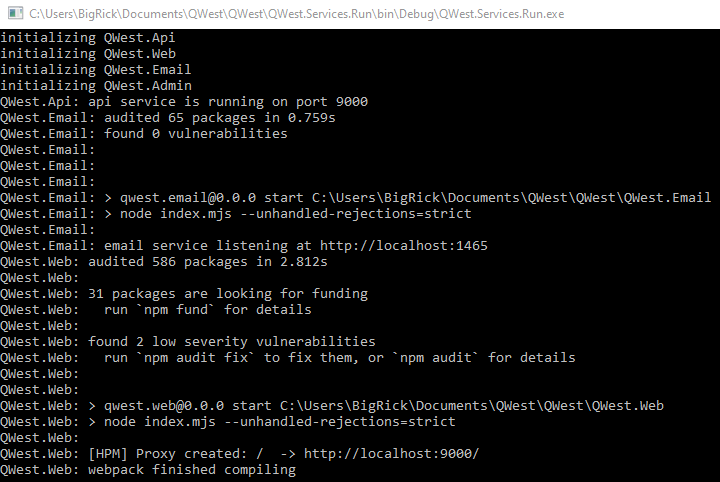
\includegraphics[width=\linewidth]{services_run_log.png}
    \caption{QWest.Services.Run opstarts log.}
    \label{fig:startup_log}
\end{figure}

Bruger-klienten tilgås gennem en browser, som sender HTTP-requests til QWest.API, der så kalder controllers til DAO til databasen. Som nævnt i sektion \ref{sec:REST} bruges der Json.NET til serialisering og JSON data til deserialisering. Da projektet er gennemført med REST, er der ingen konstant forbindelse til databasen, men i stedet laves der kun forbindelser når databasen skal opdateres ud fra en brugeroperation. 

\section{Sikkerhed}\label{sec:security}
% Security
% Identify security problems in the application, and figure out solutions. Explain identified problems, and possible solutions. 
% Keywords: SSL/TLS, Hashing, Salting, XSS, SQL Injection, CSRF, Overposting(for MVC), Man in the middle attacks, DDOS, Authentication
HTTPS vil være den primærer måde at sikre os at bruger input er sikkert enkrypteret mens de bliver transporeret til QWest.Api, .NET framework skulle have support for HTTPS. \cite{DotNetFrameworkSSL} dog har der ikke været arbejde til at sætte dette op eftersom at vi ikke ejer it SSL certificate.

For at sikre vores brugere mod leaking af deres passwords, hvis der sker et data breach, hasher og salter vi alle brugeres passwords. Der bruges \texttt{Rfc2898DeriveBytes} \cite{Rfc2898DeriveBytes} til dette. Denne klasse bruger SHA1, som er ikke er en optimal sikker hashing metode, hvilket burde ændres i næste iteration af projektet \cite{HowsecureisSHA1} til BCrypt \cite{BCrypt} eller lignende.

\section{Transactions}\label{sec:transactions}
% Transactions
% Identify places in the application where we need transactions
% How do we build our transactions? Isolation levels?
% Do we need distributed transactions?
% ACID, Parallelism, Async/Await,
% Implementation details welcome

\section{Protokoller}\label{sec:protocols}
Kommunikationen mellem alle services'ne i QWest er http requests, med untagelse af kommunikationen med databasen fra QWest.DataAccess. kommunikationen fra vores frontend web klient til QWest.Api (endten direkte eller proxiet gennem QWest.Web) skal selfølgelig være http eftersom at der ikke er webstandarder for andre muligheder, den eneste untagelse værende WebSockets, dog er dette ikke usecasen for WebSockets og WebSockets har ikke lige så stor support blandt ældrere browsere som en help normal http request har. Denne kommunikationen bruger igen JSON eftersom at frontend browser javascript ikke supporter mange andre måder at serializere og deserializere data på

Der kan argumenteres for brug af en anden type kommunikationen til og fra QWest.Email eftersom at node.js har muligheden for rå TCP og UDP, og en serializerings metode some protobuf \cite{ProtoBuf} eller binary serializering \cite{CsharpBinarySerialization} ville dette unødvendig kompleksitet ind i projektet og introdusere tredjepartsbiblioteker i enten QWest.Email eller andre services som bruger QWest.Email, derfor ender QWest.Email med at følge standarden sat af QWest.Api og bruge standard http requests der sender JSON serializeret data.

\section{Caching and HTTP optimization}\label{sec:caching}
